% Created by tikzDevice version 0.10.1 on 2019-04-12 20:09:03
% !TEX encoding = UTF-8 Unicode
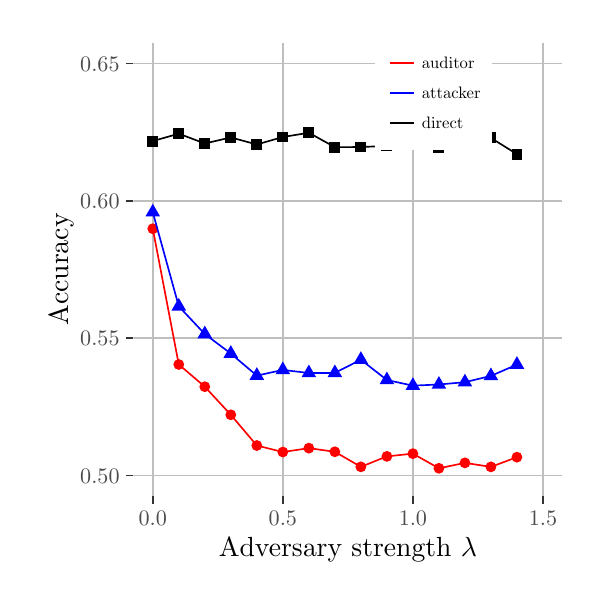
\begin{tikzpicture}[x=1pt,y=1pt]
\definecolor{fillColor}{RGB}{255,255,255}
\path[use as bounding box,fill=fillColor,fill opacity=0.00] (0,0) rectangle (198.74,198.74);
\begin{scope}
\path[clip] (  0.00,  0.00) rectangle (198.74,198.74);
\definecolor{drawColor}{RGB}{255,255,255}
\definecolor{fillColor}{RGB}{255,255,255}

\path[draw=drawColor,line width= 0.6pt,line join=round,line cap=round,fill=fillColor] ( -0.00,  0.00) rectangle (198.74,198.74);
\end{scope}
\begin{scope}
\path[clip] ( 38.16, 29.45) rectangle (193.24,193.24);
\definecolor{drawColor}{RGB}{255,255,255}

\path[draw=drawColor,line width= 0.3pt,line join=round] ( 38.16, 61.71) --
	(193.24, 61.71);

\path[draw=drawColor,line width= 0.3pt,line join=round] ( 38.16,111.34) --
	(193.24,111.34);

\path[draw=drawColor,line width= 0.3pt,line join=round] ( 38.16,160.98) --
	(193.24,160.98);

\path[draw=drawColor,line width= 0.3pt,line join=round] ( 68.70, 29.45) --
	( 68.70,193.24);

\path[draw=drawColor,line width= 0.3pt,line join=round] (115.70, 29.45) --
	(115.70,193.24);

\path[draw=drawColor,line width= 0.3pt,line join=round] (162.70, 29.45) --
	(162.70,193.24);
\definecolor{drawColor}{RGB}{190,190,190}

\path[draw=drawColor,line width= 0.6pt,line join=round] ( 38.16, 36.89) --
	(193.24, 36.89);

\path[draw=drawColor,line width= 0.6pt,line join=round] ( 38.16, 86.53) --
	(193.24, 86.53);

\path[draw=drawColor,line width= 0.6pt,line join=round] ( 38.16,136.16) --
	(193.24,136.16);

\path[draw=drawColor,line width= 0.6pt,line join=round] ( 38.16,185.80) --
	(193.24,185.80);

\path[draw=drawColor,line width= 0.6pt,line join=round] ( 45.21, 29.45) --
	( 45.21,193.24);

\path[draw=drawColor,line width= 0.6pt,line join=round] ( 92.20, 29.45) --
	( 92.20,193.24);

\path[draw=drawColor,line width= 0.6pt,line join=round] (139.20, 29.45) --
	(139.20,193.24);

\path[draw=drawColor,line width= 0.6pt,line join=round] (186.19, 29.45) --
	(186.19,193.24);
\definecolor{fillColor}{RGB}{255,0,0}

\path[fill=fillColor] ( 45.21,126.09) circle (  1.96);
\definecolor{fillColor}{RGB}{0,0,255}

\path[fill=fillColor] ( 45.21,135.11) --
	( 47.85,130.54) --
	( 42.56,130.54) --
	cycle;
\definecolor{fillColor}{RGB}{0,0,0}

\path[fill=fillColor] ( 43.24,155.79) --
	( 47.17,155.79) --
	( 47.17,159.72) --
	( 43.24,159.72) --
	cycle;
\definecolor{fillColor}{RGB}{255,0,0}

\path[fill=fillColor] ( 54.60, 77.03) circle (  1.96);
\definecolor{fillColor}{RGB}{0,0,255}

\path[fill=fillColor] ( 54.60,101.10) --
	( 57.25, 96.52) --
	( 51.96, 96.52) --
	cycle;
\definecolor{fillColor}{RGB}{0,0,0}

\path[fill=fillColor] ( 52.64,158.47) --
	( 56.57,158.47) --
	( 56.57,162.39) --
	( 52.64,162.39) --
	cycle;
\definecolor{fillColor}{RGB}{255,0,0}

\path[fill=fillColor] ( 64.00, 69.01) circle (  1.96);
\definecolor{fillColor}{RGB}{0,0,255}

\path[fill=fillColor] ( 64.00, 91.09) --
	( 66.65, 86.51) --
	( 61.36, 86.51) --
	cycle;
\definecolor{fillColor}{RGB}{0,0,0}

\path[fill=fillColor] ( 62.04,154.93) --
	( 65.97,154.93) --
	( 65.97,158.85) --
	( 62.04,158.85) --
	cycle;
\definecolor{fillColor}{RGB}{255,0,0}

\path[fill=fillColor] ( 73.40, 58.85) circle (  1.96);
\definecolor{fillColor}{RGB}{0,0,255}

\path[fill=fillColor] ( 73.40, 84.03) --
	( 76.05, 79.46) --
	( 70.76, 79.46) --
	cycle;
\definecolor{fillColor}{RGB}{0,0,0}

\path[fill=fillColor] ( 71.44,157.11) --
	( 75.37,157.11) --
	( 75.37,161.03) --
	( 71.44,161.03) --
	cycle;
\definecolor{fillColor}{RGB}{255,0,0}

\path[fill=fillColor] ( 82.80, 47.75) circle (  1.96);
\definecolor{fillColor}{RGB}{0,0,255}

\path[fill=fillColor] ( 82.80, 76.06) --
	( 85.44, 71.49) --
	( 80.16, 71.49) --
	cycle;
\definecolor{fillColor}{RGB}{0,0,0}

\path[fill=fillColor] ( 80.84,154.57) --
	( 84.76,154.57) --
	( 84.76,158.49) --
	( 80.84,158.49) --
	cycle;
\definecolor{fillColor}{RGB}{255,0,0}

\path[fill=fillColor] ( 92.20, 45.40) circle (  1.96);
\definecolor{fillColor}{RGB}{0,0,255}

\path[fill=fillColor] ( 92.20, 78.12) --
	( 94.84, 73.54) --
	( 89.56, 73.54) --
	cycle;
\definecolor{fillColor}{RGB}{0,0,0}

\path[fill=fillColor] ( 90.24,157.26) --
	( 94.16,157.26) --
	( 94.16,161.19) --
	( 90.24,161.19) --
	cycle;
\definecolor{fillColor}{RGB}{255,0,0}

\path[fill=fillColor] (101.60, 46.80) circle (  1.96);
\definecolor{fillColor}{RGB}{0,0,255}

\path[fill=fillColor] (101.60, 77.01) --
	(104.24, 72.43) --
	( 98.96, 72.43) --
	cycle;
\definecolor{fillColor}{RGB}{0,0,0}

\path[fill=fillColor] ( 99.64,158.80) --
	(103.56,158.80) --
	(103.56,162.72) --
	( 99.64,162.72) --
	cycle;
\definecolor{fillColor}{RGB}{255,0,0}

\path[fill=fillColor] (111.00, 45.49) circle (  1.96);
\definecolor{fillColor}{RGB}{0,0,255}

\path[fill=fillColor] (111.00, 77.04) --
	(113.64, 72.46) --
	(108.36, 72.46) --
	cycle;
\definecolor{fillColor}{RGB}{0,0,0}

\path[fill=fillColor] (109.04,153.61) --
	(112.96,153.61) --
	(112.96,157.53) --
	(109.04,157.53) --
	cycle;
\definecolor{fillColor}{RGB}{255,0,0}

\path[fill=fillColor] (120.40, 40.05) circle (  1.96);
\definecolor{fillColor}{RGB}{0,0,255}

\path[fill=fillColor] (120.40, 81.83) --
	(123.04, 77.25) --
	(117.76, 77.25) --
	cycle;
\definecolor{fillColor}{RGB}{0,0,0}

\path[fill=fillColor] (118.44,153.64) --
	(122.36,153.64) --
	(122.36,157.56) --
	(118.44,157.56) --
	cycle;
\definecolor{fillColor}{RGB}{255,0,0}

\path[fill=fillColor] (129.80, 43.83) circle (  1.96);
\definecolor{fillColor}{RGB}{0,0,255}

\path[fill=fillColor] (129.80, 74.47) --
	(132.44, 69.90) --
	(127.16, 69.90) --
	cycle;
\definecolor{fillColor}{RGB}{0,0,0}

\path[fill=fillColor] (127.84,154.06) --
	(131.76,154.06) --
	(131.76,157.98) --
	(127.84,157.98) --
	cycle;
\definecolor{fillColor}{RGB}{255,0,0}

\path[fill=fillColor] (139.20, 44.81) circle (  1.96);
\definecolor{fillColor}{RGB}{0,0,255}

\path[fill=fillColor] (139.20, 72.44) --
	(141.84, 67.86) --
	(136.55, 67.86) --
	cycle;
\definecolor{fillColor}{RGB}{0,0,0}

\path[fill=fillColor] (137.24,156.01) --
	(141.16,156.01) --
	(141.16,159.94) --
	(137.24,159.94) --
	cycle;
\definecolor{fillColor}{RGB}{255,0,0}

\path[fill=fillColor] (148.60, 39.52) circle (  1.96);
\definecolor{fillColor}{RGB}{0,0,255}

\path[fill=fillColor] (148.60, 72.85) --
	(151.24, 68.27) --
	(145.95, 68.27) --
	cycle;
\definecolor{fillColor}{RGB}{0,0,0}

\path[fill=fillColor] (146.63,153.36) --
	(150.56,153.36) --
	(150.56,157.28) --
	(146.63,157.28) --
	cycle;
\definecolor{fillColor}{RGB}{255,0,0}

\path[fill=fillColor] (158.00, 41.48) circle (  1.96);
\definecolor{fillColor}{RGB}{0,0,255}

\path[fill=fillColor] (158.00, 73.69) --
	(160.64, 69.11) --
	(155.35, 69.11) --
	cycle;
\definecolor{fillColor}{RGB}{0,0,0}

\path[fill=fillColor] (156.03,154.43) --
	(159.96,154.43) --
	(159.96,158.36) --
	(156.03,158.36) --
	cycle;
\definecolor{fillColor}{RGB}{255,0,0}

\path[fill=fillColor] (167.39, 40.03) circle (  1.96);
\definecolor{fillColor}{RGB}{0,0,255}

\path[fill=fillColor] (167.39, 75.95) --
	(170.04, 71.37) --
	(164.75, 71.37) --
	cycle;
\definecolor{fillColor}{RGB}{0,0,0}

\path[fill=fillColor] (165.43,156.94) --
	(169.36,156.94) --
	(169.36,160.86) --
	(165.43,160.86) --
	cycle;
\definecolor{fillColor}{RGB}{255,0,0}

\path[fill=fillColor] (176.79, 43.54) circle (  1.96);
\definecolor{fillColor}{RGB}{0,0,255}

\path[fill=fillColor] (176.79, 80.05) --
	(179.44, 75.47) --
	(174.15, 75.47) --
	cycle;
\definecolor{fillColor}{RGB}{0,0,0}

\path[fill=fillColor] (174.83,151.08) --
	(178.76,151.08) --
	(178.76,155.00) --
	(174.83,155.00) --
	cycle;
\definecolor{drawColor}{RGB}{255,0,0}

\path[draw=drawColor,line width= 0.6pt,line join=round] ( 45.21,126.09) --
	( 54.60, 77.03) --
	( 64.00, 69.01) --
	( 73.40, 58.85) --
	( 82.80, 47.75) --
	( 92.20, 45.40) --
	(101.60, 46.80) --
	(111.00, 45.49) --
	(120.40, 40.05) --
	(129.80, 43.83) --
	(139.20, 44.81) --
	(148.60, 39.52) --
	(158.00, 41.48) --
	(167.39, 40.03) --
	(176.79, 43.54);
\definecolor{drawColor}{RGB}{0,0,255}

\path[draw=drawColor,line width= 0.6pt,line join=round] ( 45.21,132.06) --
	( 54.60, 98.05) --
	( 64.00, 88.04) --
	( 73.40, 80.98) --
	( 82.80, 73.01) --
	( 92.20, 75.07) --
	(101.60, 73.96) --
	(111.00, 73.99) --
	(120.40, 78.77) --
	(129.80, 71.42) --
	(139.20, 69.39) --
	(148.60, 69.80) --
	(158.00, 70.64) --
	(167.39, 72.90) --
	(176.79, 77.00);
\definecolor{drawColor}{RGB}{0,0,0}

\path[draw=drawColor,line width= 0.6pt,line join=round] ( 45.21,157.76) --
	( 54.60,160.43) --
	( 64.00,156.89) --
	( 73.40,159.07) --
	( 82.80,156.53) --
	( 92.20,159.23) --
	(101.60,160.76) --
	(111.00,155.57) --
	(120.40,155.60) --
	(129.80,156.02) --
	(139.20,157.98) --
	(148.60,155.32) --
	(158.00,156.40) --
	(167.39,158.90) --
	(176.79,153.04);
\end{scope}
\begin{scope}
\path[clip] (  0.00,  0.00) rectangle (198.74,198.74);
\definecolor{drawColor}{gray}{0.30}

\node[text=drawColor,anchor=base east,inner sep=0pt, outer sep=0pt, scale=  0.80] at ( 33.21, 34.14) {0.50};

\node[text=drawColor,anchor=base east,inner sep=0pt, outer sep=0pt, scale=  0.80] at ( 33.21, 83.77) {0.55};

\node[text=drawColor,anchor=base east,inner sep=0pt, outer sep=0pt, scale=  0.80] at ( 33.21,133.41) {0.60};

\node[text=drawColor,anchor=base east,inner sep=0pt, outer sep=0pt, scale=  0.80] at ( 33.21,183.04) {0.65};
\end{scope}
\begin{scope}
\path[clip] (  0.00,  0.00) rectangle (198.74,198.74);
\definecolor{drawColor}{gray}{0.20}

\path[draw=drawColor,line width= 0.6pt,line join=round] ( 35.41, 36.89) --
	( 38.16, 36.89);

\path[draw=drawColor,line width= 0.6pt,line join=round] ( 35.41, 86.53) --
	( 38.16, 86.53);

\path[draw=drawColor,line width= 0.6pt,line join=round] ( 35.41,136.16) --
	( 38.16,136.16);

\path[draw=drawColor,line width= 0.6pt,line join=round] ( 35.41,185.80) --
	( 38.16,185.80);
\end{scope}
\begin{scope}
\path[clip] (  0.00,  0.00) rectangle (198.74,198.74);
\definecolor{drawColor}{gray}{0.20}

\path[draw=drawColor,line width= 0.6pt,line join=round] ( 45.21, 26.70) --
	( 45.21, 29.45);

\path[draw=drawColor,line width= 0.6pt,line join=round] ( 92.20, 26.70) --
	( 92.20, 29.45);

\path[draw=drawColor,line width= 0.6pt,line join=round] (139.20, 26.70) --
	(139.20, 29.45);

\path[draw=drawColor,line width= 0.6pt,line join=round] (186.19, 26.70) --
	(186.19, 29.45);
\end{scope}
\begin{scope}
\path[clip] (  0.00,  0.00) rectangle (198.74,198.74);
\definecolor{drawColor}{gray}{0.30}

\node[text=drawColor,anchor=base,inner sep=0pt, outer sep=0pt, scale=  0.80] at ( 45.21, 18.99) {0.0};

\node[text=drawColor,anchor=base,inner sep=0pt, outer sep=0pt, scale=  0.80] at ( 92.20, 18.99) {0.5};

\node[text=drawColor,anchor=base,inner sep=0pt, outer sep=0pt, scale=  0.80] at (139.20, 18.99) {1.0};

\node[text=drawColor,anchor=base,inner sep=0pt, outer sep=0pt, scale=  0.80] at (186.19, 18.99) {1.5};
\end{scope}
\begin{scope}
\path[clip] (  0.00,  0.00) rectangle (198.74,198.74);
\definecolor{drawColor}{RGB}{0,0,0}

\node[text=drawColor,anchor=base,inner sep=0pt, outer sep=0pt, scale=  1.00] at (115.70,  7.70) {Adversary strength $\lambda$};
\end{scope}
\begin{scope}
\path[clip] (  0.00,  0.00) rectangle (198.74,198.74);
\definecolor{drawColor}{RGB}{0,0,0}

\node[text=drawColor,rotate= 90.00,anchor=base,inner sep=0pt, outer sep=0pt, scale=  1.00] at ( 14.59,111.34) {Accuracy};
\end{scope}
\begin{scope}
\path[clip] (  0.00,  0.00) rectangle (198.74,198.74);
\definecolor{fillColor}{RGB}{255,255,255}

\path[fill=fillColor] (125.54,154.53) rectangle (167.90,199.20);
\end{scope}
\begin{scope}
\path[clip] (  0.00,  0.00) rectangle (198.74,198.74);
\definecolor{drawColor}{RGB}{255,0,0}

\path[draw=drawColor,line width= 0.6pt,line join=round] (130.89,185.90) -- (139.56,185.90);
\end{scope}
\begin{scope}
\path[clip] (  0.00,  0.00) rectangle (198.74,198.74);
\definecolor{drawColor}{RGB}{0,0,255}

\path[draw=drawColor,line width= 0.6pt,line join=round] (130.89,175.06) -- (139.56,175.06);
\end{scope}
\begin{scope}
\path[clip] (  0.00,  0.00) rectangle (198.74,198.74);
\definecolor{drawColor}{RGB}{0,0,0}

\path[draw=drawColor,line width= 0.6pt,line join=round] (130.89,164.22) -- (139.56,164.22);
\end{scope}
\begin{scope}
\path[clip] (  0.00,  0.00) rectangle (198.74,198.74);
\definecolor{drawColor}{RGB}{0,0,0}

\node[text=drawColor,anchor=base west,inner sep=0pt, outer sep=0pt, scale=  0.60] at (142.45,183.83) {auditor};
\end{scope}
\begin{scope}
\path[clip] (  0.00,  0.00) rectangle (198.74,198.74);
\definecolor{drawColor}{RGB}{0,0,0}

\node[text=drawColor,anchor=base west,inner sep=0pt, outer sep=0pt, scale=  0.60] at (142.45,172.99) {attacker};
\end{scope}
\begin{scope}
\path[clip] (  0.00,  0.00) rectangle (198.74,198.74);
\definecolor{drawColor}{RGB}{0,0,0}

\node[text=drawColor,anchor=base west,inner sep=0pt, outer sep=0pt, scale=  0.60] at (142.45,162.15) {direct};
\end{scope}
\end{tikzpicture}
